\documentclass{beamer} 

\mode<presentation> {
    \usetheme{ARAMIS}
}

\usepackage[english]{babel}
\usepackage[utf8]{inputenc}

\usepackage{amsmath,amsthm, amssymb, latexsym}
\usefonttheme[onlymath]{serif}
\boldmath

\usepackage[orientation=portrait,size=a0,scale=1.4,debug]{beamerposter}           % e.g. for DIN-A0 poster
%\usepackage[orientation=portrait,size=a1,scale=1.4,grid,debug]{beamerposter}     % e.g. for DIN-A1 poster, with optional grid and debug output
%\usepackage[size=custom,width=200,height=120,scale=2,debug]{beamerposter}        % e.g. for custom size poster
%\usepackage[orientation=portrait,size=a0,scale=1.0,printer=rwth-glossy-uv.df]{beamerposter}     % e.g. for DIN-A0 poster with rwth-glossy-uv printer check
% ...
%
\usepackage{tcolorbox}
\tcbset{%
    noparskip,
    colback=white, %background color of the box
    colframe=normalTitleBlockColor, %color of frame and title background
    coltext=black, %color of body text
    coltitle=black, %color of title text 
    %fonttitle=\bfseries,
    %valign upper=center,
    %boxsep=2mm,
    boxrule=1.5mm,
    alerted/.style={coltitle=red, 
                     colframe=gray!40},
    example/.style={coltitle=black, 
                     colframe=green!20,             
                     colback=green!5},
    }

\usepackage{tikz}
\usetikzlibrary{arrows,snakes,backgrounds,patterns,matrix,shapes,fit,calc,shadows,plotmarks,intersections,shapes.geometric}

\beamertemplatenavigationsymbolsempty

\usepackage{xspace}
\newcommand{\TODO}{{\color{red}\bf [TODO]}}
\newcommand{\cybersec}{cybersecurity\xspace}
\newcommand{\Cybersec}{Cybersecurity\xspace}
\newcommand{\aramis}{Aramis\xspace}
\newcommand{\DiH}{Diffie-Hellman\xspace}
\newcommand{\XOR}{Exclusive-Or\xspace}
\newcommand{\modbus}{MODBUS\xspace}
\newcommand{\opcua}{OPC-UA\xspace}

\graphicspath{{assets/}}
\makeatletter
    \def\input@path{{assets/}}
\makeatother

\title{Attack Traffic Generation Against SCADA Systems}
\author{Maxime Puys, Marie-Laure Potet and Jean-Louis Roch}
\institute{VERIMAG, University of Grenoble Alpes, France}
\date{}

\begin{document}
\begin{frame}[t]
        \begin{columns}[T]
            \begin{column}{.49\textwidth}
                \begin{tcolorbox}[adjusted title={\centering\large Industrial Systems}]
                    \centering
                    \vspace{1.1em}
                    \begin{columns}
                        \begin{column}{.3\textwidth}
                            \resizebox{\textwidth}{!}{
                                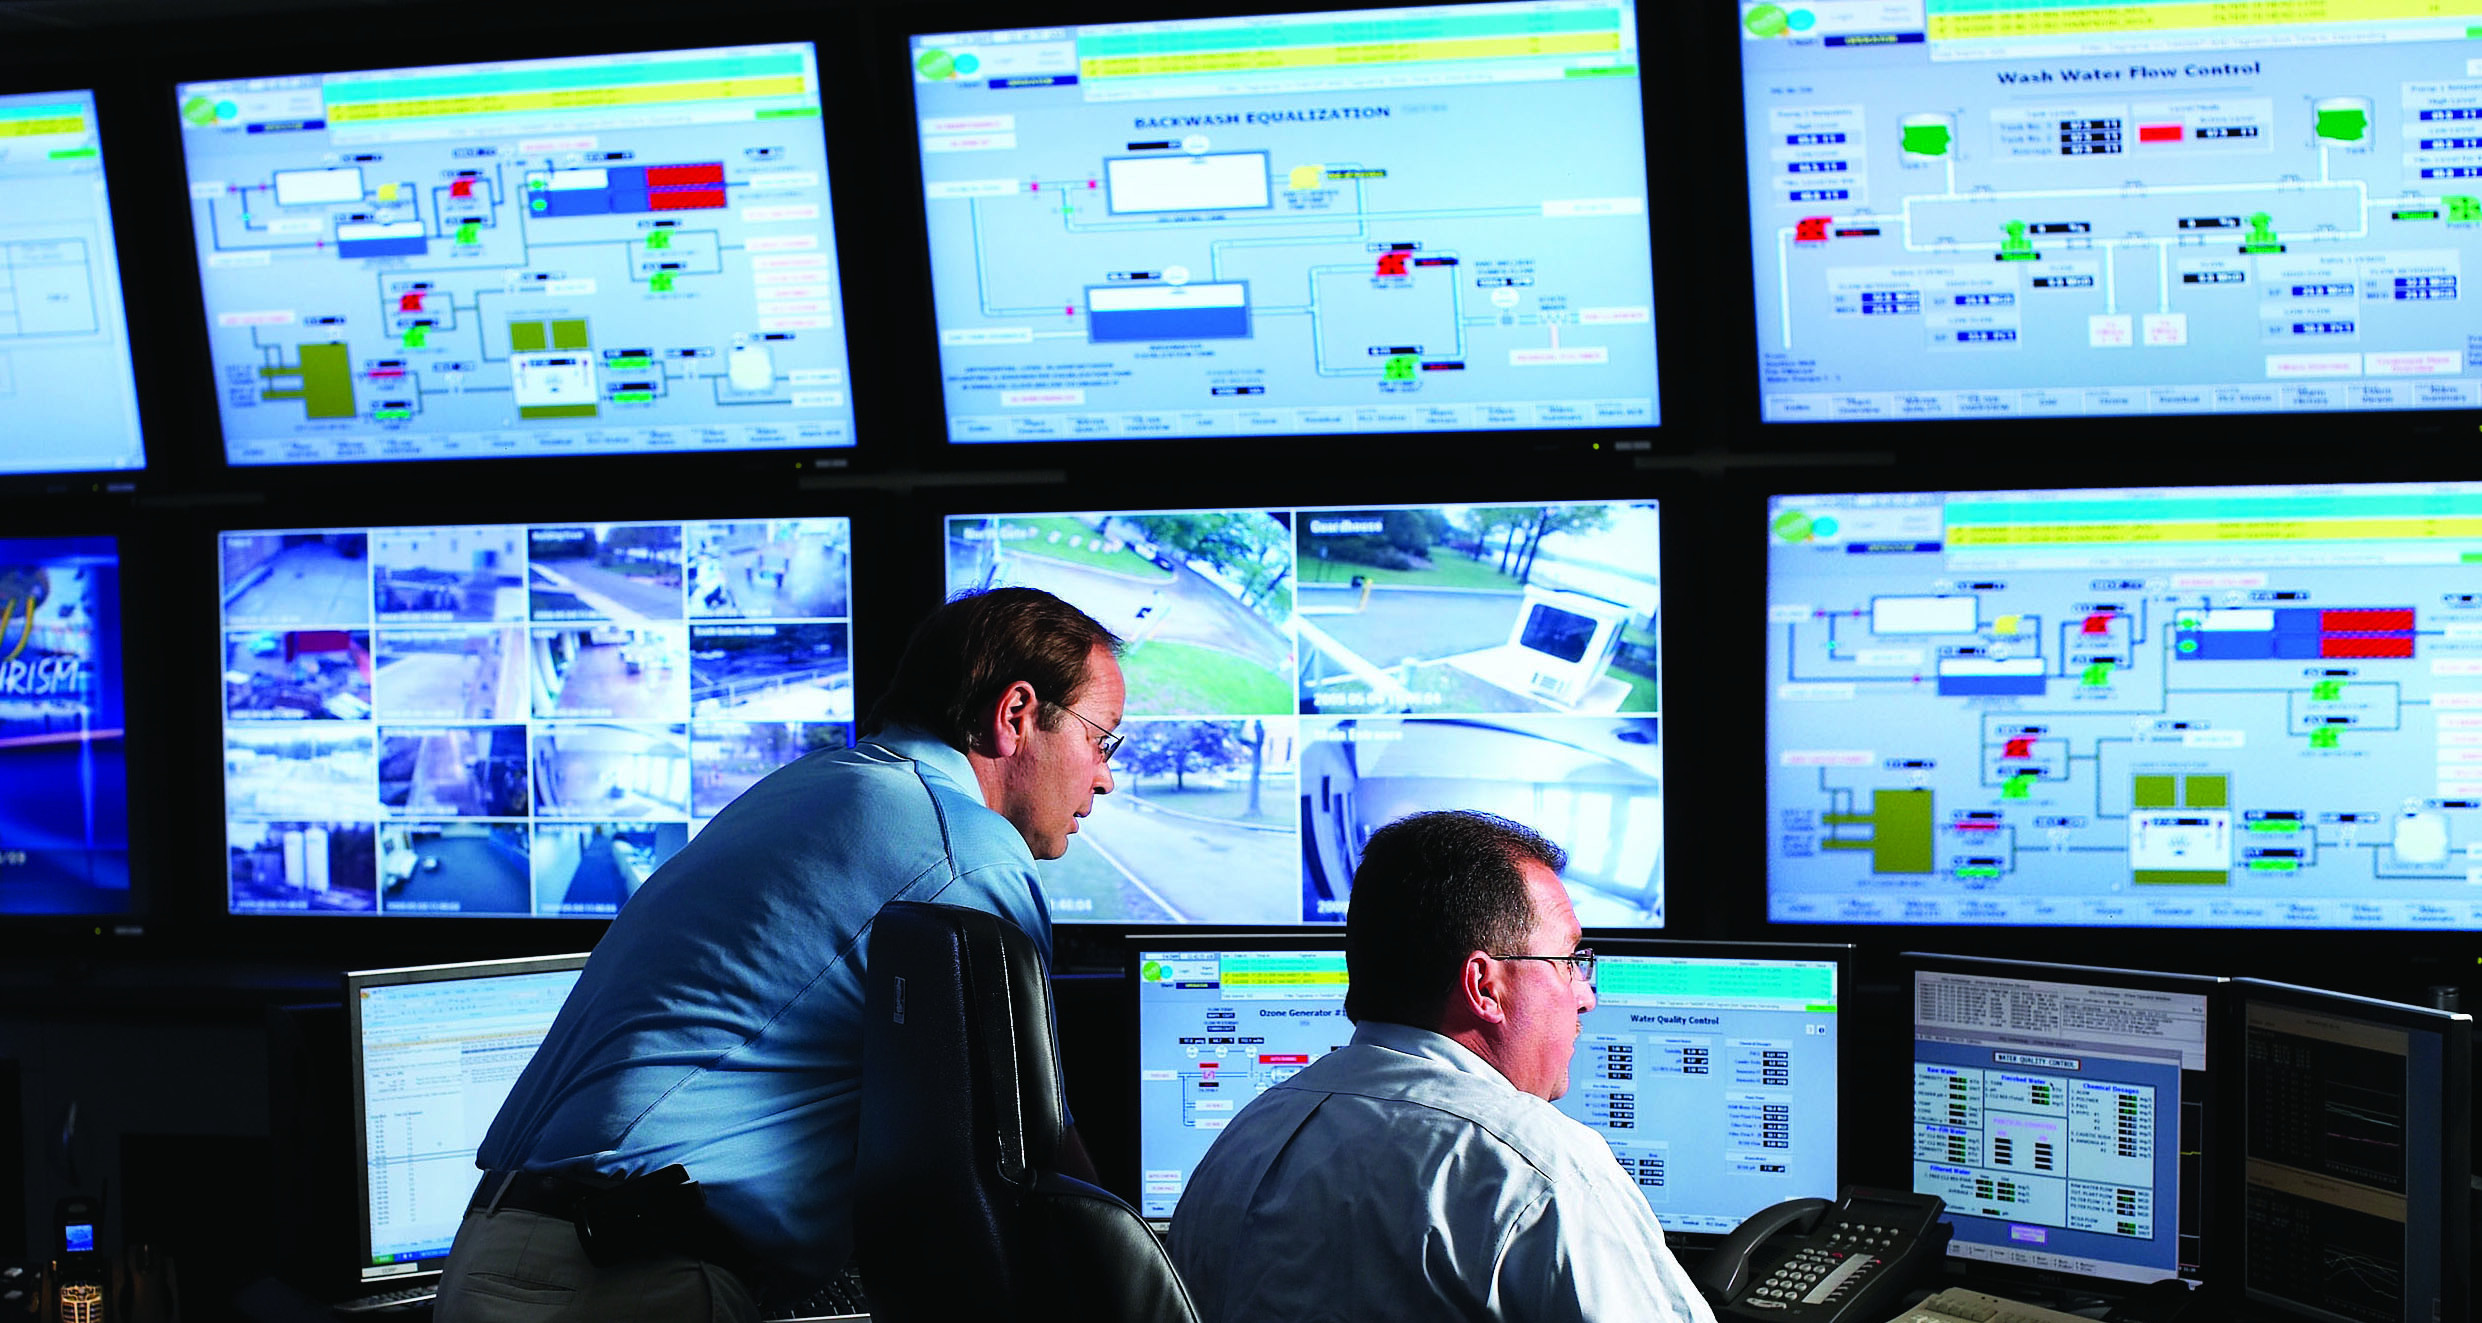
\includegraphics{scada}
                            }
                        \end{column}
                        \begin{column}{.3\textwidth}
                            \resizebox{\textwidth}{!}{
                                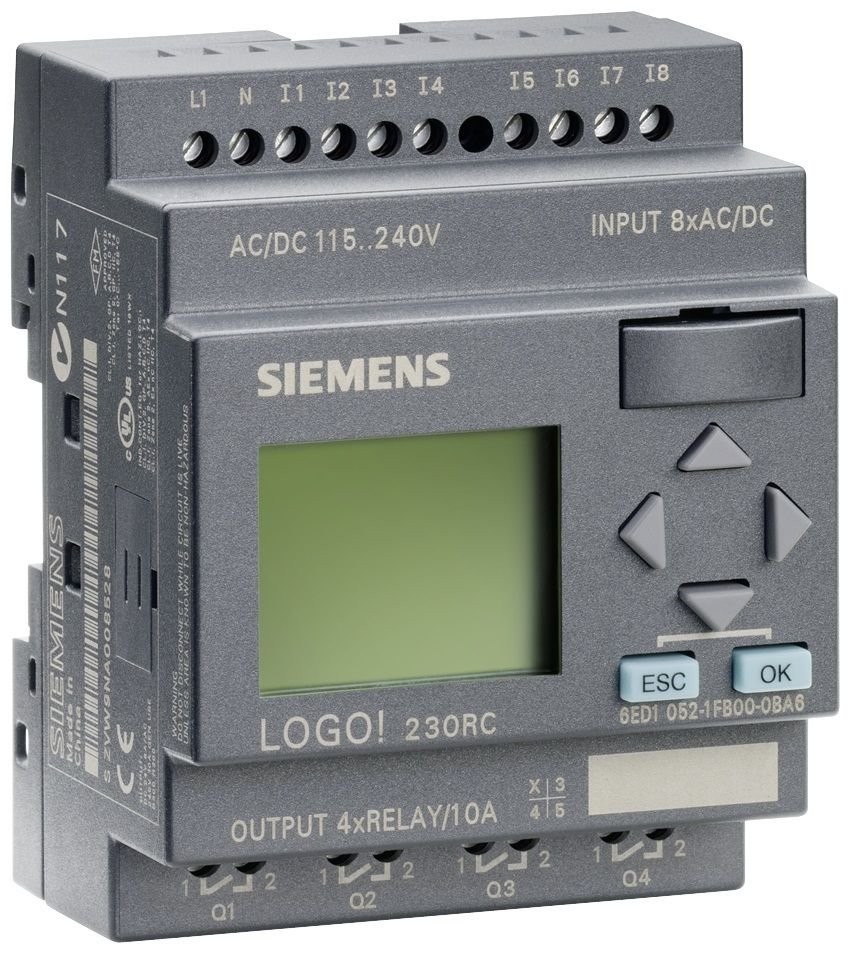
\includegraphics{plc}
                            }
                        \end{column}
                        \begin{column}{.3\textwidth}
                            \resizebox{\textwidth}{!}{
                                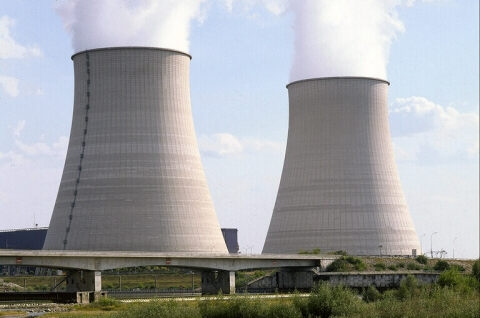
\includegraphics{plant}
                            }
                        \end{column}
                    \end{columns}
                    \vspace{1.1em}
                    \begin{itemize}
                        \item Increasing number of attacks showed in the medias since Stuxnet \cite{Lan11}.
                        \item Becoming a priority for government agencies.
                        \begin{itemize}
                            \item LPM to ensure the security of OIVs.
                            \item Publications from ANSSI, DGA, ...
                        \end{itemize}
                    \end{itemize}
                \end{tcolorbox}
            \end{column}
            %\hfill
            \begin{column}{.49\textwidth}
                \begin{tcolorbox}[adjusted title={\centering\large Security concepts}]
                    \begin{itemize}
                        \item Safety = Protection against identified/natural difficulties.
                        \begin{itemize}
                            \item Historic industrial concern.
                        \end{itemize}
                        \item \Cybersec = Protection against malicious adversaries.
                        \begin{itemize}
                            \item Often called Security.
                        \end{itemize}
                    \end{itemize}

                    \begin{figure}[htb]
                        \resizebox{.85\columnwidth}{!}{
                            \def\rectangle{(-1.5,-4.5) rectangle (12,5.25)}
\def\secondcircle{(0:15.75) ellipse (6 and 4.5)}
\def\thridcircle{(0:-5.25) ellipse (6 and 4.5)}
\def\fourthcircle{(0:5.25) ellipse (6.75 and 3)}

\begin{tikzpicture}
    \draw \rectangle node at (5.25,4) {Industrial systems};
    \draw \secondcircle node {\Cybersec};
    \draw \thridcircle node {Safety};
    \draw \fourthcircle node [align=center]{Industrial \\ systems \\ \cybersec};
    \begin{scope}[fill opacity=0.25]
        \fill[blue]   \rectangle;
        \fill[red]    \secondcircle;
        \fill[green]  \thridcircle;
        \fill[yellow] \fourthcircle;
    \end{scope}
\end{tikzpicture}

                        }
                        \vspace{-.2cm}
                        \caption{Relations among security concepts}
                    \end{figure}
                    \vspace{-.5cm}
                    \begin{itemize}
                        \item Ludovic Pietre-Cambacedes' thesis: On the relationships between safety and security, Telecom ParisTech and EDF, 2010.
                    \end{itemize}
                \end{tcolorbox}
            \end{column}
        \end{columns}
        \vfill
        \begin{tcolorbox}[adjusted title={\centering\large Objectives}]
            \begin{itemize}
                \item Modelize SCADA infrastructures (components, network links and communication protocols) and their threats (in terms of position, capacities and objectives),
                \item From a modelling, automaticaly produce abstract attack scenarios that an adversary should follow to achieve one of his objective,
                \item Convert them to real network packets able to launch the attack on a platform to verify and quantify their plausibility.
            \end{itemize}
        \end{tcolorbox}
        \vfill
        \begin{tcolorbox}[adjusted title={\centering\large Approach}]
            \begin{columns}[T]
                \begin{column}{.35\textwidth}
                    \begin{figure}[htb]
                        \resizebox{\columnwidth}{!}{
                            \begin{tikzpicture}[
        arrow/.style={thick,->,shorten >=2pt,shorten <=2pt,>=stealth},
    ]
    \draw (2,6) rectangle (5,7) node [pos=.5] {Architecture};
    \draw (6,6) rectangle (9,7) node [pos=.5] {Prop. de sécurité};


    \draw (4,4) rectangle (7,5) node [pos=.5] {Analyses};

    \draw (0,2) rectangle (3,3) node [pos=.5] {Bibliothèque};
    \draw (4,0) rectangle (7,1) node [pos=.5] {Paquets};
    \draw (8,2) rectangle (11,3) node [pos=.5] {Contexte};

    \draw (4,2) rectangle (7,3) node [align=center,pos=.5] {Instanciation\\Concrétisation};

    \draw[arrow] (3.5,6) -- (5.5,5); % Archi --> Analyses
    \draw[arrow] (7.5,6) -- (5.5,5); % Props --> Analyses
    \draw[arrow] (5.5,4) -- (5.5,3) node [pos=.5,right] {Suite d'actions décrivant des attaques}; % Analyses --> Inst
    \draw[arrow] (3,2.5) -- (4,2.5); % Biblio --> Inst
    \draw[arrow] (8,2.5) -- (7,2.5); % Context--> Inst
    \draw[arrow] (5.5,2) -- (5.5,1); % Inst --> Packets
\end{tikzpicture}

                        }
                        \vspace{-1.5cm}
                        \caption{Our global approach}
                    \end{figure}
                \end{column}
                \begin{column}{.64\textwidth}
                \end{column}
            \end{columns}
        \end{tcolorbox}
        \vfill
    \end{frame}
\end{document}

